\section{Full SLAM}

In the general case, we encounter:
\[\Pr(x_t,m|z_t)\neq \Pr(x_t|z_t)\Pr(m|z_t)\]
This disparity arises due to the correlation between position and pose.
However, when considering the entire trajectory $X_t$ rather than just a single pose $x_t$, we find:
\[\Pr(X_t,m|z_t)\neq \Pr(X_t|z_t)\Pr(m|X_t,z_t)\]
Thus, in this scenario, the map becomes independent of the current state.
In FastSLAM, the trajectory $X_t$ is represented by particles $X_t^{(i)}$, while the map is represented by a factorization known as the Rao-Blackwellized Filter:
\[\Pr\left(m|X_t^{(i)},z_t\right)=\prod_j^M\Pr\left(m_j|X_t^{(i)},z_t\right)\]
Here, $\Pr\left(X_t|z_t\right)$ is computed using particles, and $\Pr\left(m|X_t,z_t\right)$ is estimated using an Extended Kalman Filter.

To decouple the map of features from poses, each particle represents a robot trajectory. 
Feature measurements are correlated throughout the robot trajectory.
If the robot trajectory is known, all features would be uncorrelated. 
Treat each pose particle as if it is the true trajectory, processing all feature measurements independently.

\paragraph*{SLAM posterior}
The factored posterior is given by:
\begin{align*}
    \Pr(x_{1:t},l_{1:m}|z_{1:t},u_{0:t-1})  &=\Pr(x_{1:t}|z_{1:t},u_{0:t-1})\Pr(l_{1:m}|x_{1:t},z_{1:t}) \\
                                            &=\Pr(x_{1:t}|z_{1:t},u_{0:t-1})\prod_{i=1}^{M}\Pr(l_{i}|x_{1:t},z_{1:t})
\end{align*}
Here, $\Pr(x_{1:t}|z_{1:t},u_{0:t-1})$ represents the robot path posterior (localization problem), and $\Pr(l_{i}|x_{1:t},z_{1:t})$ denotes the conditionally independent landmark positions. 
The dimension of conditionally independent landmark positions is $m$.

\subsection{FastSLAM}
In practice, FastSLAM is implemented via Rao-Blackwellized particle filtering based on landmarks. 
Each particle represents a trajectory, consisting of the last pose and a reference to the previous one. 
Each landmark is represented by a $2\times 2$ Extended Kalman Filter (EKF). 
Therefore, each particle needs to maintain $M$ EKFs.
\begin{figure}[H]
    \centering
    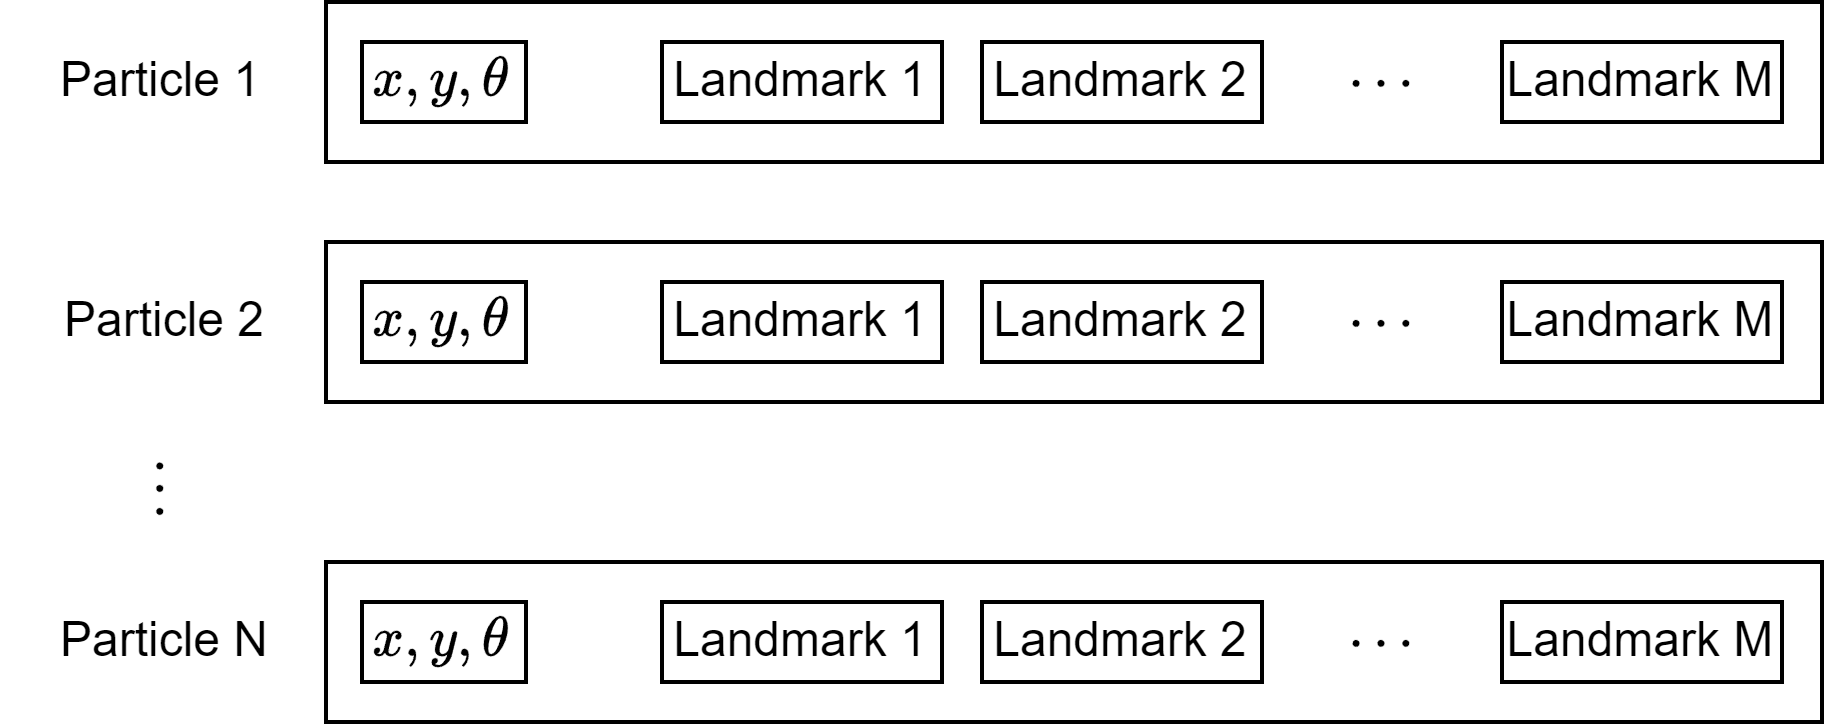
\includegraphics[width=0.75\linewidth]{images/fast.png}
    \caption{Particles in FastSLAM}
\end{figure}

\paragraph*{Complexity}
The update of the robot particles depends on the number of particles $N$, leading to a complexity of $\mathcal{O}(N)$. 
Incorporating observations into the Kalman filter involves updating a section of the map features $M$, resulting in a complexity of $\mathcal{O}(N\log M)$. 
Resampling the particle set also requires the same complexity of $\mathcal{O}(N\log M)$. 
Therefore, the total complexity of the algorithm is:
\[\mathcal{O}(N\log M)\]
Here, $N$ is the number of particles, and $M$ is the number of map features.

\paragraph{Improvements}
Since each particle contains a map of the entire environment, and each grid is independent from the others, we can select the best map at each time by updating all the maps.